% 第2章：数学基础
\section{数学基础}
\label{sec:math}

\subsection{克利福德代数 $\Cl(3,1)$ 与 $Cl(1,9)$ 的对偶}

我们方法的基础在于克利福德代数，它为描述旋量和时空几何提供了自然的代数框架。

\subsubsection{四维时空代数 $\Cl(3,1)$}

\begin{definition}[克利福德代数 $\Cl(3,1)$]
克利福德代数 $\Cl(3,1)$ 是由 $\{\gamma^0, \gamma^1, \gamma^2, \gamma^3\}$ 生成的在 $\mathbb{R}$ 上的结合代数，关系为：
\begin{equation}
    \{\gamma^\mu, \gamma^\nu\} = 2\eta^{\mu\nu} \mathbf{1}
\end{equation}
其中 $\eta^{\mu\nu} = \diag(-1, 1, 1, 1)$ 是闵可夫斯基度规。
\end{definition}

该代数的维度为 $2^4 = 16$，分解为：
\begin{equation}
    \Cl(3,1) \cong \text{Mat}(4, \mathbb{R})
\end{equation}

基由以下给出：
\begin{align}
    \&\{1\} \u0026\u0026 \text{（1个标量）} \\
    \&\{\gamma^\mu\} \u0026\u0026 \text{（4个矢量）} \\
    \&\{\gamma^{\mu\nu} = \gamma^{[\mu}\gamma^{\nu]}\} \u0026\u0026 \text{（6个双向量）} \\
    \&\{\gamma^{\mu\nu\rho} = \gamma^{[\mu}\gamma^\nu\gamma^{\rho]}\} \u0026\u0026 \text{（4个三向量）} \\
    \&\{\gamma^{0123} = \gamma_5\} \u0026\u0026 \text{（1个伪标量）}
\end{align}

\subsubsection{十维内空间代数 $Cl(1,9)$}

\begin{definition}[克利福德代数 $Cl(1,9)$]
克利福德代数 $Cl(1,9)$ 由 $\{\Gamma^0, \Gamma^1, ..., \Gamma^9\}$ 生成，关系为：
\begin{equation}
    \{\Gamma^A, \Gamma^B\} = 2\eta^{AB} \mathbf{1}
\end{equation}
其中 $\eta^{AB} = \diag(-1, 1, 1, 1, 1, 1, 1, 1, 1, 1)$。
\end{definition}

$Cl(1,9)$ 的维度为 $2^{10} = 1024$，包含32×32矩阵表示。

\subsubsection{两种代数的对偶关系}

\begin{insight}[$\Cl(3,1)$ 与 $Cl(1,9)$ 的界面]
第\ref{sec:four_forces_unified}章将详细讨论，两种代数通过4维时空与10维内空间的\textbf{界面}形成对偶：
\begin{itemize}
    \item $\Cl(3,1)$ 描述可观测的4维互反空间
    \item $Cl(1,9)$ 描述高维内空间的几何结构
    \item 扭转场 $\torsion^\alpha_{\ \mu\nu}$ 作为界面场连接两者
\end{itemize}
\end{insight}

\subsection{自旋群与覆盖映射}

自旋群 $\Spin(3,1)$ 是真时向洛伦兹群 $SO^+(3,1)$ 的二重覆盖：
\begin{equation}
    \rho: \Spin(3,1) \to SO^+(3,1)
\end{equation}

核为 $\ker(\rho) = \{+1, -1\} = Z_2$。

\begin{theorem}[万有覆盖]
映射 $\rho$ 是万有覆盖同态，使 $\Spin(3,1)$ 成为 $SO^+(3,1)$ 的万有覆盖群。
\end{theorem}

类似地，$\Spin(1,9)$ 是 $SO^+(1,9)$ 的二重覆盖。

\subsection{谱维}

谱维提供了一个有效的维度概念，可以随能量尺度变化。

\begin{definition}[谱维]
对于黎曼流形 $(M, g)$，谱维通过热核迹定义：
\begin{equation}
    Z(t) = \Tr(e^{t\Delta})
\end{equation}
其中 $\Delta$ 是拉普拉斯-贝尔特拉米算子。在尺度 $\ell = \sqrt{t}$ 的谱维为：
\begin{equation}
    d_s(\ell) = -2 \frac{d \ln Z(t)}{d \ln t}
\end{equation}
\end{definition}

在我们的框架中，谱维从普朗克尺度的 $d_s = 10$ 跑到宏观尺度的 $d_s = 4$：
\begin{equation}
    d_s(T) = 4 + \frac{6}{1 + (T/T_c)^2}
\end{equation}

其中 $T_c \sim 10^{16}$ GeV 是GUT能标。

\begin{figure}[htbp]
\centering
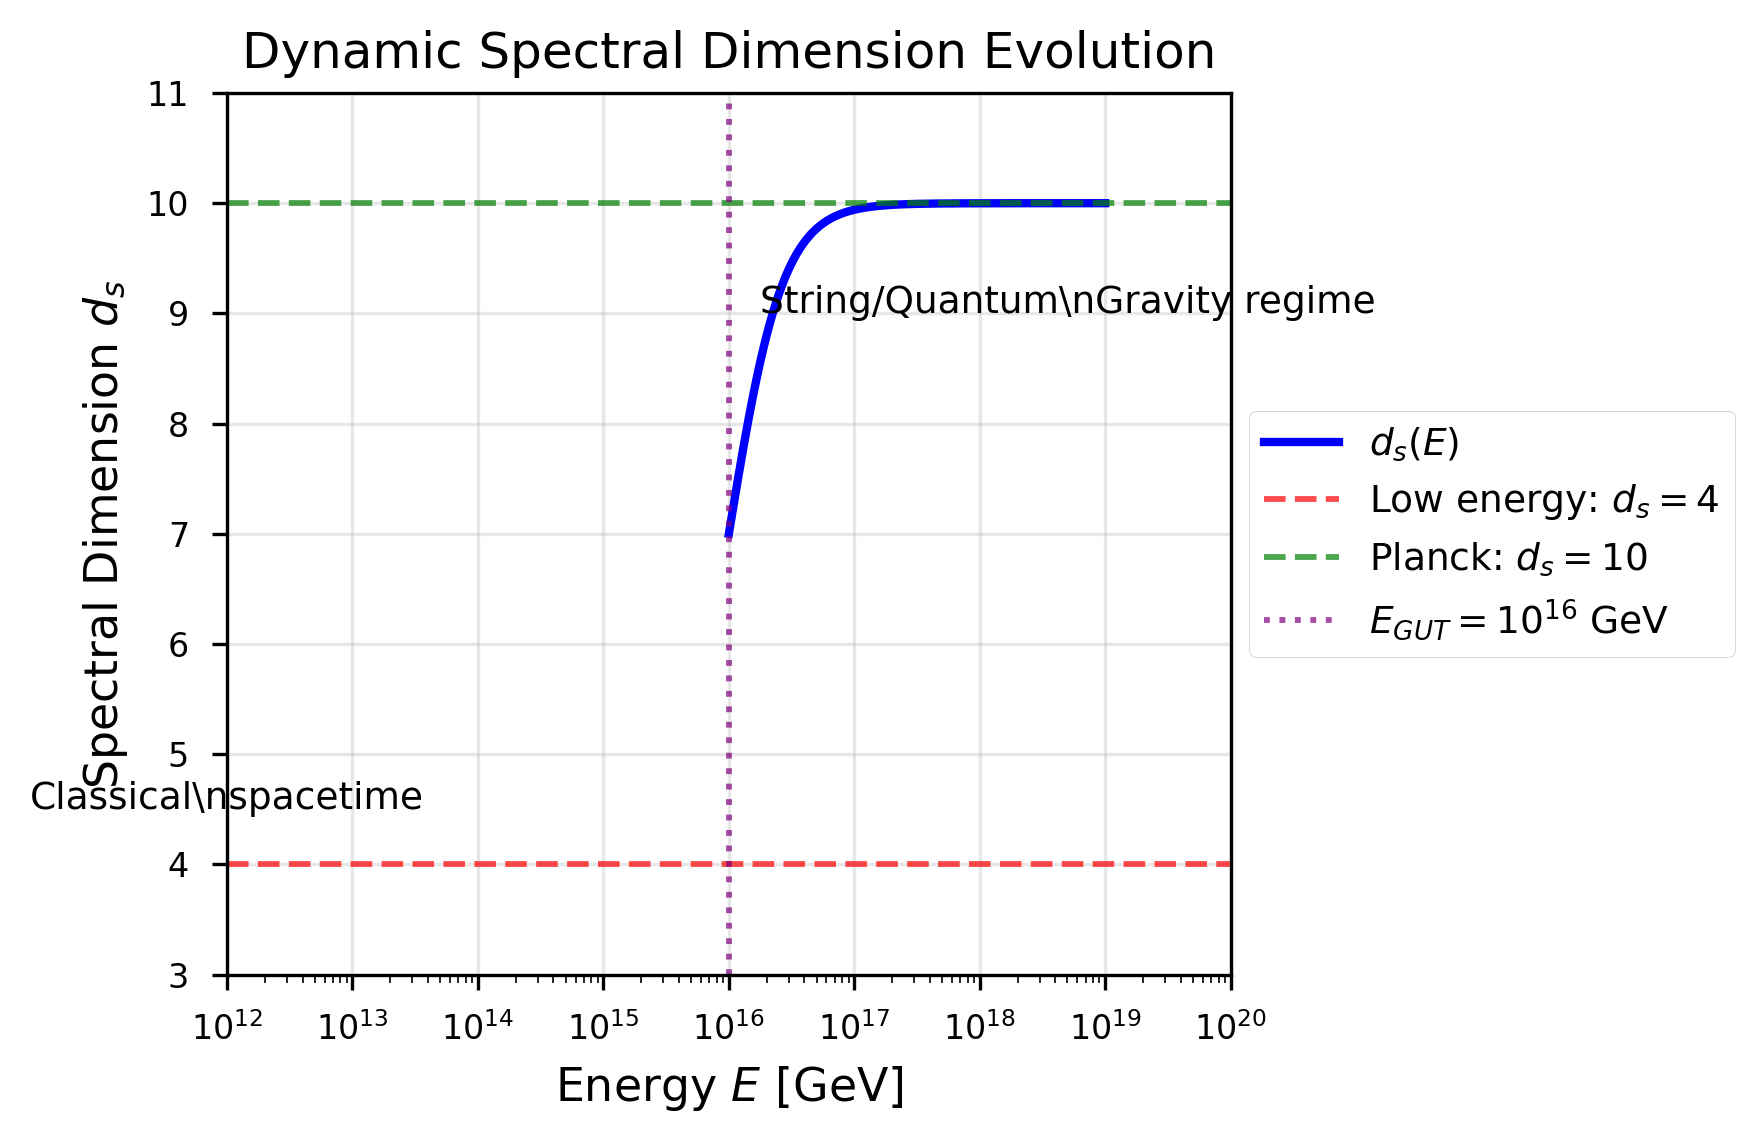
\includegraphics[width=0.8\textwidth]{figures/fig1_spectral_dimension.png}
\caption{动态谱维演化。在高能（$T \gg T_c$），谱维接近10，而在低能它冻结为4。}
\label{fig:spectral_dimension}
\end{figure}

\subsection{分形测度}

豪斯多夫维度 $d_H$ 和谱维 $d_s$ 表征了小尺度时空的分形结构。

\begin{definition}[分形测度]
集合 $S$ 上的分形测度定义为：
\begin{equation}
    \mu_\alpha(S) = \lim_{\delta \to 0} \inf \left\{\sum_i (\text{diam } U_i)^\alpha : S \subseteq \bigcup_i U_i, \text{diam } U_i < \delta\right\}
\end{equation}
豪斯多夫维度是临界值 $\alpha = d_H$，其中 $\mu_\alpha$ 从 $\infty$ 跳到 $0$。
\end{definition}

对于具有动态谱维的时空，我们推广：
\begin{equation}
    d_{eff}(\ell) = d_s(\ell)
\end{equation}

\subsection{扭转克利福德代数}

关键创新是通过扭转克利福德代数引入扭转。

\begin{definition}[扭转自旋群]
扭转自旋群 $\Spin^\tau(3,1)$ 通过修改覆盖映射以包含扭转来定义：
\begin{equation}
    \rho^\tau: \Spin^\tau(3,1) \to SO^\tau(3,1)
\end{equation}
其中 $SO^\tau(3,1)$ 是带扭转的洛伦兹群。
\end{definition}

扭转场的几何解释为时空的扭曲提供了物理内涵。

\subsection{与规范理论的关联}

扭转克利福德代数自然包含规范对称性：
\begin{equation}
    \Spin^\tau(3,1) \supset SU(2) \times U(1) \subset SO(6)
\end{equation}

这将在第\ref{sec:gauge}章详细展开。

\subsection{总结}

本章介绍了UFT的数学基础：
\begin{enumerate}
    \item \textbf{克利福德代数}：$\Cl(3,1)$ 描述4维时空，$Cl(1,9)$ 描述10维内空间
    \item \textbf{对偶关系}：两种代数通过扭转场界面相互对偶
    \item \textbf{谱维}：有效维度随能量尺度从10流动到4
    \item \textbf{分形结构}：小尺度时空具有分形几何
    \item \textbf{扭转}：通过扭转克利福德代数引入，携带物理意义
\end{enumerate}

这些数学工具为后续构建统一场论提供了坚实的基础。
